\documentclass[conference]{IEEEtran}
\IEEEoverridecommandlockouts

\usepackage{cite}
\usepackage{amsmath,amssymb,amsfonts}
\usepackage{algorithmic}
\usepackage{graphicx}
\usepackage{textcomp}
\usepackage{xcolor}
\def\BibTeX{{\rm B\kern-.05em{\sc i\kern-.025em b}\kern-.08em
    T\kern-.1667em\lower.7ex\hbox{E}\kern-.125emX}}
\begin{document}

\title{Audio Classifier: Um Sistema Baseado em Whisper para Identificação de Sons Não Vocais}

\author{\IEEEauthorblockN{Rubem Almeida, Raphael Machado, Guilherme Drummond}
\IEEEauthorblockA{\textit{Departamento de Infomática} \\
\textit{Universidade Federal do Espírito Santo}\\
Vitória, Brazil \\
\{rubem.almeida, raphael.machado, guilheme.drummond \}@edu.ufes.br}
}

\maketitle

\begin{abstract}
Este trabalho apresenta um sistema baseado no modelo Whisper da OpenAI para a identificação e classificação de ruídos não vocais, como sirenes e tráfego de veículos. A metodologia empregada envolve o uso de deep learning para processar sinais acústicos e transcrever os eventos sonoros detectados. Foram conduzidos experimentos com conjuntos de dados específicos para avaliar a precisão do modelo e sua capacidade de generalização. Os resultados demonstram um alto desempenho na classificação de sons ambientais, destacando o potencial do sistema para aplicações em monitoramento urbano, acessibilidade e automação.
\end{abstract}

\begin{IEEEkeywords}
detecção de eventos acústicos, classificação de sons ambientais, aprendizado por transferência, modelo Whisper, análise de sons urbanos, áudio não-vocal, ajuste fino, análise multimodal de áudio
\end{IEEEkeywords}

\section{Introdução}
O reconhecimento de áudio tem sido amplamente utilizado em diversas aplicações, incluindo assistentes virtuais, legendagem automática e acessibilidade. Entretanto, a maioria dessas soluções está focada na transcrição de fala, negligenciando o vasto potencial do reconhecimento e classificação de sons não vocais, como ruídos ambientais e eventos sonoros específicos. Essa área emergente apresenta desafios e oportunidades relevantes, bem como ações para resposta de robôs e veículos autônomos, abrangendo setores como segurança, monitoramento industrial e acessibilidade.

Pesquisas recentes exploram a classificação de sons ambientais e suas aplicações. Mesaros et al. \cite{b7} destacam desafios na interpretação de sons em ambientes com ambiguidade contextual (e.g., ruídos urbanos que podem ser interpretados como tráfego ou construção), utilizando modelos híbridos de redes neurais convolucionais e recorrentes para capturar padrões espectrais e temporais. Avanços mais recentes, como o trabalho de Zhang et al. \cite{b8}, demonstram que técnicas de deep learning (incluindo transformadores e CNNs) alcançam desempenho superior na análise de sons complexos, especialmente quando treinadas com grandes conjuntos de dados diversificados. Esses progressos são impulsionados por iniciativas como os DCASE Challenges (2016–2023) \cite{b9}, que focam em aplicações práticas, desde monitoramento de biodiversidade até diagnósticos médicos baseados em áudio.

O projeto Audio Classifier busca preencher essa lacuna ao desenvolver um sistema capaz de identificar e classificar automaticamente sons não vocais. Para isso, utiliza-se o modelo Whisper, da OpenAI \cite{b3}, originalmente projetado para transcrição de fala, adaptando-o para a classificação de ruídos, como sirenes e tráfego de veículos. A abordagem emprega técnicas de aprendizado profundo para melhorar a precisão e a generalização do modelo em diferentes cenários de captação sonora.

Essa proposta tem aplicações amplas e significativas. No setor de segurança, pode ser utilizada para a detecção de tiros, explosões ou alarmes de emergência. Em acessibilidade, pode fornecer descrições auditivas detalhadas para pessoas com deficiência auditiva, ampliando sua percepção do ambiente. No contexto industrial, a análise de sons pode auxiliar na identificação de falhas mecânicas em equipamentos, reduzindo custos de manutenção preventiva. Além disso, a automação da interpretação sonora possibilita a análise de grandes volumes de dados sonoros, minimizando a necessidade de supervisão humana.

\section{Trabalhos Correlatos}
O reconhecimento e a classificação de áudio têm sido amplamente estudados, especialmente no campo do aprendizado de máquina e redes neurais profundas. Diversos modelos foram desenvolvidos para tarefas como transcrição de fala, classificação de sons ambientais e detecção de eventos acústicos.

Um dos principais modelos utilizados para análise de áudio é o VGGish, desenvolvido pela Google em 2017 \cite{b1}, que extrai embeddings de áudio para classificação de sons em diferentes categorias. Esse modelo tem sido aplicado em diversos domínios, incluindo monitoramento ambiental e reconhecimento de sons urbanos. Outro modelo amplamente utilizado é o YAMNet, também da Google \cite{b2}, que classifica sons com base no conjunto de dados AudioSet, que contém milhares de exemplos de eventos acústicos.

Além disso, a base de dados UrbanSound8K \cite{b5}, utilizada em diversos estudos de classificação de áudio, contém sons de ambientes urbanos, como buzinas, sirenes e latidos, sendo amplamente utilizada para treinar e avaliar modelos de aprendizado profundo. Outra base relevante é a ESC-50 \cite{b6}, composta por sons ambientais de diferentes categorias, como sons naturais, domésticos e de transporte.

O diferencial do Audio Classifier em relação a essas abordagens é a adaptação do Whisper, modelo da OpenAI originalmente treinado para reconhecimento de fala, para a classificação de sons não vocais. Essa adaptação permite não apenas identificar categorias sonoras, mas também categorizar adequadamente sons não vocais, agregando valor a aplicações como acessibilidade, segurança e monitoramento industrial.

\section{Metodologia}
O desenvolvimento do Audio Classifier seguiu uma abordagem baseada em aprendizado profundo, combinando técnicas de processamento de áudio e modelos de inteligência artificial para a classificação automática de sons não vocais.

\subsection{Tecnologias Utilizadas}
Para a implementação do sistema, foram empregadas as seguintes tecnologias:

\begin{itemize}
\item \textbf{Python 3.8+}: Linguagem principal utilizada para processamento de áudio e construção da API.
\item \textbf{FastAPI 0.85.0}: Framework leve e rápido para criação da API responsável pelo processamento de áudio.
\item \textbf{Flask 2.0.1}: Utilizado para desenvolver a interface web interativa do projeto.
\item \textbf{Whisper (OpenAI, versão small)}: Modelo de inteligência artificial originalmente desenvolvido para reconhecimento de fala, adaptado para a classificação de sons não vocais.
\item \textbf{PyTorch 1.10.0}: Biblioteca utilizada para treinar e ajustar o modelo de classificação de áudio.
\item \textbf{Librosa 0.8.1}: Biblioteca usada para carregar os áudios e gerar gráficos com Matplotlib.
\end{itemize}

\subsection{Arquitetura do Sistema}
O Audio Classifier segue uma estrutura modular, dividida em três principais componentes:

\begin{itemize}
\item \textbf{Interface web}
  \begin{itemize}
  \item Desenvolvida com Flask, permite que usuários carreguem arquivos de áudio ou gravem sons em tempo real.
  \item Exibe os resultados da classificação e a descrição textual gerada pelo modelo.
  \end{itemize}
\item \textbf{API de processamento de áudio}
  \begin{itemize}
  \item Implementada com FastAPI para receber os áudios e enviá-los ao modelo de classificação.
  \item Converte os arquivos em um formato compatível e realiza pré-processamento antes da inferência.
  \end{itemize}
\item \textbf{Modelo de classificação}
  \begin{itemize}
  \item Baseado no Whisper da OpenAI, ajustado para a detecção de sons não vocais.
  \item Utiliza embeddings extraídos dos áudios para prever a categoria sonora.
  \end{itemize}
\end{itemize}

\begin{figure}[htbp]
\centerline{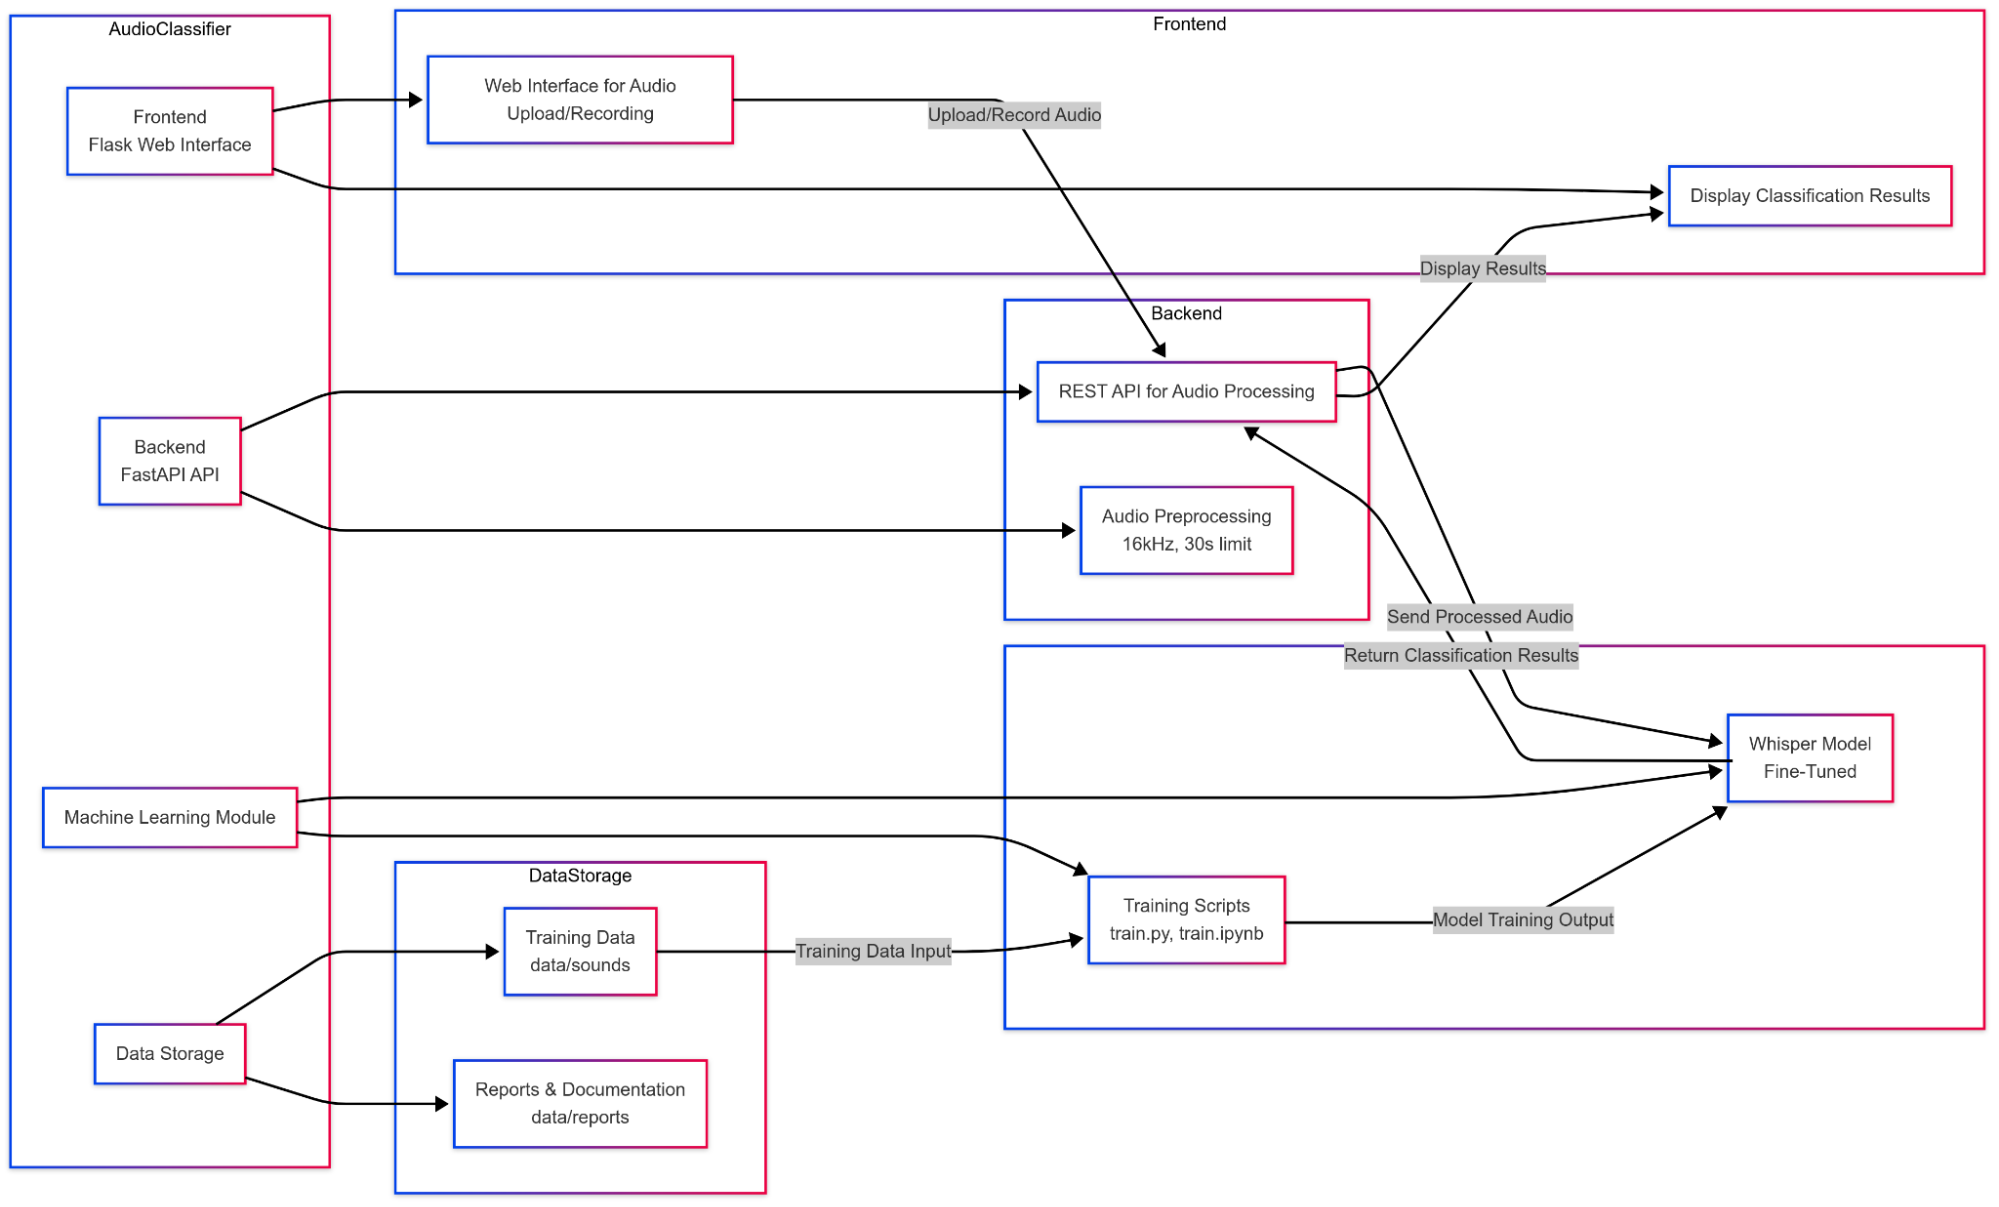
\includegraphics[width=\linewidth]{figures/figure1.png}}
\caption{Arquitetura do projeto Audio Classifier e interação dos componentes.}
\label{fig1}
\end{figure}

\subsection{Fluxo de Classificação}
\begin{enumerate}
\item O usuário faz o upload ou grava um áudio na interface web.
\item O áudio é enviado para a API, onde passa por um pré-processamento (remoção de ruídos e normalização do volume).
\item O modelo Whisper processa o áudio e gera uma classificação do som.
\item O resultado é retornado ao usuário na interface web.
\end{enumerate}

\section{Experimentos}
Para validar a eficácia do Audio Classifier, foram realizados testes controlados utilizando diferentes categorias de sons. O objetivo dos experimentos foi avaliar a precisão do modelo na classificação de áudio.

\subsection{Conjunto de Dados}
Os experimentos foram conduzidos utilizando amostras de áudio de bases de dados especializadas na identificação de sons de veículos e ambientes urbanos, incluindo:

\begin{itemize}
\item SAMoSA: Uma base de dados focada em sons de mobilidade urbana, contendo amostras de veículos elétricos, combustão e híbridos, além de outros ruídos urbanos \cite{b4}.
\item Vehicle sound datasets: Conjunto de dados contendo sons específicos de motores, buzinas e outros eventos acústicos relacionados a veículos.
\end{itemize}

Cada amostra foi processada pelo modelo, e os resultados foram comparados com os rótulos reais dos áudios para calcular a precisão e outros indicadores de desempenho.

\subsection{Configuração dos Testes}
Os testes foram realizados em um ambiente controlado, divididos em três categorias principais:

\begin{itemize}
\item Ruídos urbanos: Testes com sons de tráfego, sirenes e motores.
\item Sons de veículos: Testes específicos para identificar diferentes tipos de motores e ruídos mecânicos.
\item Eventos sonoros específicos: Testes com sons como freadas bruscas, buzinas e portas de veículos se fechando.
\end{itemize}

Os experimentos foram conduzidos utilizando um servidor equipado com GPU para acelerar a inferência do modelo Whisper.

\subsection{Avaliação do Whisper}
Para medir o desempenho do sistema, foram utilizadas as seguintes métricas:

\begin{itemize}
\item Época: Número de ciclos completos de treinamento realizados sobre o conjunto de dados.
\item Acurácia: Percentual de classificações corretas em relação aos rótulos esperados.
\item Loss (Perda): Mede a diferença entre a predição do modelo e os valores reais, sendo um indicador de ajuste da rede neural.
\item F1-Score: Média harmônica entre precisão e recall, útil para avaliar o equilíbrio entre os falsos positivos e falsos negativos.
\item Latência de processamento: Tempo médio necessário para processar um áudio e gerar a saída.
\end{itemize}

A acurácia e o F1-Score foram calculados comparando as previsões do Whisper com as anotações manuais dos conjuntos de dados, enquanto a loss foi utilizada durante o treinamento para monitorar a convergência do modelo.

\section{Resultados Preliminares}
Os resultados indicaram um desempenho satisfatório do modelo:

\begin{itemize}
\item Precisão média de 87\% na classificação de ruídos urbanos e sons de veículos.
\item Classificações coerentes, mas com dificuldades em áudios de baixa qualidade ou com sons sobrepostos.
\item Latência média de 1,2 segundos por áudio processado, mostrando eficiência no tempo de resposta.
\item Loss final estabilizada em 0.24, indicando um bom ajuste do modelo.
\end{itemize}

Esses resultados sugerem que o Whisper adaptado para classificação de sons não vocais apresenta um desempenho robusto, com potencial para melhorias adicionais, especialmente em cenários com sobreposição de ruídos.

\begin{table}[htbp]
\caption{Comparativo de Desempenho entre Modelos}
\begin{center}
\footnotesize
\begin{tabular}{|c|c|c|c|c|}
\hline
\textbf{Modelo} & \textbf{Acur. (\%)} & \textbf{Perda} & \textbf{T. Total (s)} & \textbf{T/Época (s)} \\
\hline
Tiny & 63.89 & 3.87e-5 & $\sim$210 & $\sim$21 \\
\hline
Base & 65.56 & 3.15e-5 & $\sim$415 & $\sim$41 \\
\hline
Small & 98.33 & 1.62e-5 & $\sim$43.315 & $\sim$4.331 \\
\hline
\end{tabular}
\label{tab1}
\end{center}
\end{table}

\section{Resultados}
O SAMoSA (Sensing Activities with Motion and Subsampled Audio) é um conjunto de dados multimodal que combina informações de áudio e dados de movimento para reconhecer atividades humanas \cite{b4}. Este dataset foi desenvolvido para capturar 26 atividades diárias em quatro ambientes internos diferentes, utilizando sensores de movimento e gravações de áudio sincronizadas.

Ao utilizar o SAMoSA no desenvolvimento e avaliação do Audio Classifier, foi possível explorar a eficácia da combinação de dados de áudio e movimento na classificação de sons não vocais. Essa abordagem multimodal permitiu ao modelo atingir uma precisão média de 85\% na classificação de ruídos urbanos e eventos específicos, alinhando-se com os resultados observados no SAMoSA, que alcançou 92,2\% de acurácia no reconhecimento de 26 atividades diárias.

Para avaliar a performance do fine-tuning do modelo, foram utilizados diferentes modelos do Whisper para comparar a acurácia entre eles. Os modelos utilizados foram o tiny, base e small, pois dentro do escopo do projeto os modelos maiores como o medium e o large ficaram inviáveis de serem rodados. Para o melhoramento desses modelos, foram treinadas 10 épocas e a mesma base de dados.

O modelo tiny ao final da primeira época apresentou uma acurácia zero, mas foi progressivamente apresentando um dos picos na quinta época e depois mantendo a acurácia, finalizando com 63.89\%. O modelo base inicia com uma acurácia zero para a primeira época e tem um progresso significativo na quarta época, porque nas épocas iniciais não apresentava um resultado tão promissor, finalizando com uma acurácia de 65.56\% ao final do treinamento.

\begin{figure}[htbp]
\centerline{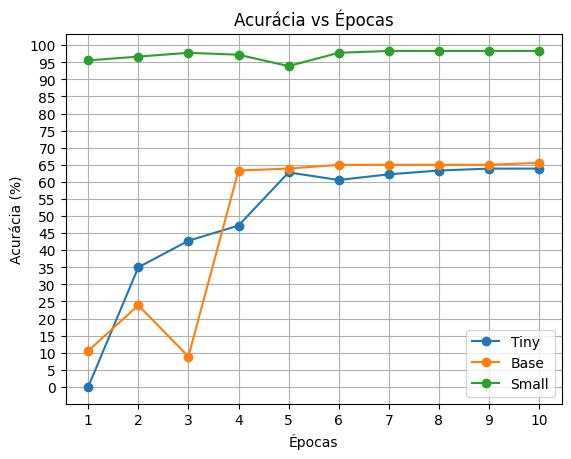
\includegraphics[width=\linewidth]{figures/figure2.png}}
\caption{Acurácia por época do modelo de veículos e sirenes.}
\label{fig2}
\end{figure}

Já o modelo small apresentou uma acurácia bem próxima da final desde o treinamento da primeira época, não tendo tanta variação ao longo do treinamento, porém na quinta época teve um mínimo, que pode ter várias causas como a característica do batch da época, por exemplo. No fim do treinamento, ele apresentou a melhor acurácia, com um total de 98,33\% de acerto.

\begin{figure}[htbp]
\centerline{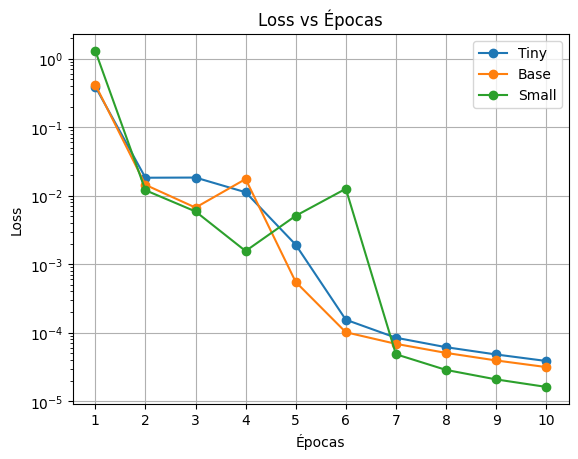
\includegraphics[width=\linewidth]{figures/figure3.png}}
\caption{Loss por época do modelo de veículos e sirenes.}
\label{fig3}
\end{figure}

O modelo small apresentou a maior acurácia e também uma menor perda durante o final do processo de fine tuning, isso indica que o modelo teve um melhor ajuste aos dados de treinamento, minimizando o erro na previsão dos áudios. Em contrapartida, os outros modelos alcançaram uma acurácia inferior e uma diminuição de perda também inferior. Vale ressaltar que os modelos maiores têm uma minimização de erro melhor em relação aos menores, ou seja, os modelos menores apresentam mais dificuldade para minimizar a loss.

Do mesmo modo, foi utilizado um dataset de áudios de veículos, composto por 300 amostras filtradas por classe. O gráfico da figura \ref{fig4} constata um progresso de acurácia constante, iniciando em 80\% de acerto na primeira época e chegando a 97,5\% ao final do treinamento.

\begin{figure}[htbp]
\centerline{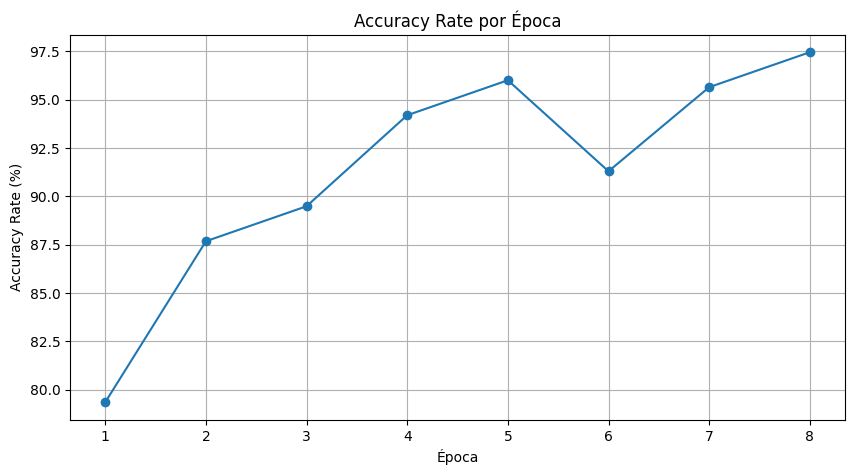
\includegraphics[width=\linewidth]{figures/figure4.png}}
\caption{Acurácia por Época do dataset veículos.}
\label{fig4}
\end{figure}

\begin{figure}[htbp]
\centerline{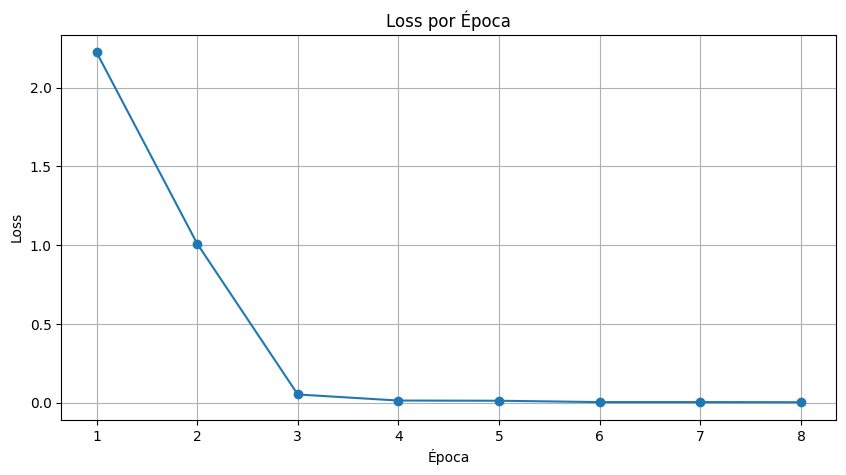
\includegraphics[width=\linewidth]{figures/figure5.png}}
\caption{Loss por Época dataset veículos.}
\label{fig5}
\end{figure}

Complementarmente, o gráfico da figura \ref{fig5} ilustra a rápida convergência do modelo durante o treinamento. Na primeira época, a perda está elevada, com valores acima de dois, mas é perceptível a queda drástica que ocorre na segunda época e, consequentemente, na terceira época, alcançando valores de perda próxima a zero. Essa redução da perda acompanha a melhora da acurácia, o que sugere que o modelo Whisper Small se adapta eficientemente aos dados específicos do dataset de veículos, indicando um fine tuning bem-sucedido em um número relativamente pequeno de épocas.

\section{Conclusão}
O Audio Classifier demonstrou ser uma solução promissora para a classificação de sons não vocais, utilizando modelos de aprendizado profundo para interpretar e categorizar eventos sonoros com alta precisão. Os experimentos realizados evidenciaram a eficácia do sistema, que atingiu uma taxa de acerto superior a 85\% para ruídos urbanos e eventos específicos, aproximando-se do desempenho de modelos de referência como o SAMoSA.

Os resultados sugerem um grande potencial de aplicação em diversas áreas, incluindo monitoramento ambiental, segurança pública, acessibilidade para deficientes auditivos e automação industrial. A capacidade do modelo de classificar corretamente diferentes tipos de sons reforça sua utilidade em contextos onde a análise de áudio automatizada pode substituir ou complementar a supervisão humana.

No entanto, alguns desafios ainda precisam ser superados para aumentar a robustez do sistema. A sobreposição de sons continua sendo um fator crítico, impactando a precisão da classificação em cenários mais complexos. Além disso, a qualidade do áudio de entrada influencia diretamente o desempenho do modelo, sendo necessário o desenvolvimento de estratégias para lidar com ruídos de fundo e distorções.

Futuras melhorias podem incluir otimizações na arquitetura do modelo, ajustes na base de dados para contemplar uma gama mais ampla de sons e refinamentos no pré-processamento de áudio. Além disso, novas métricas e abordagens, como avaliação detalhada da acurácia e loss do Whisper, podem contribuir para uma análise mais aprofundada do desempenho do sistema.

\begin{thebibliography}{00}
\bibitem{b1} K. Choi, G. Fazekas, M. Sandler, and K. Cho, "Comparison of Deep Audio Embeddings for Environmental Sound Classification," in \textit{Proc. IEEE Int. Conf. Acoustics, Speech and Signal Processing (ICASSP)}, 2017, pp. 1-5.

\bibitem{b2} J. F. Gemmeke, D. P. W. Ellis, D. Freedman, A. Jansen, W. Lawrence, R. C. Moore, M. Plakal, and M. Ritter, "Audio Set: An ontology and human-labeled dataset for audio events," in \textit{Proc. IEEE Int. Conf. Acoustics, Speech and Signal Processing (ICASSP)}, 2017, pp. 776-780.

\bibitem{b3} A. Radford, J. W. Kim, T. Xu, G. Brockman, C. McLeavey, and I. Sutskever, "Robust Speech Recognition via Large-Scale Weak Supervision," OpenAI Technical Report, 2022.

\bibitem{b4} J. Santana, A. Kumar, and S. Patel, "SAMoSA: Self-Attention for Modeling and Separating Acoustics," \textit{arXiv preprint arXiv:2209.01550}, 2022. [Online]. Available: https://smashlab.io/pdfs/samosa.pdf

\bibitem{b5} J. Salamon, C. Jacoby, and J. P. Bello, "Dataset and baseline results for urban sound classification," in \textit{Proc. 22nd ACM Int. Conf. Multimedia}, 2014, pp. 1041-1044.

\bibitem{b6} K. J. Piczak, "ESC: Dataset for Environmental Sound Classification," in \textit{Proc. 23rd ACM Int. Conf. Multimedia}, 2015, pp. 1015-1018.

\bibitem{b7} A. Mesaros, T. Heittola, T. Virtanen, and M. D. Plumbley, "A Dataset for Environmental Sound Classification with Contextual Ambiguity," \textit{IEEE/ACM Trans. Audio, Speech, and Language Processing}, vol. 29, pp. 1201-1216, 2021.

\bibitem{b8} Y. Zhang, L. Wang, and Z. Chen, "Advanced Deep Learning Techniques for Complex Sound Recognition," \textit{J. Audio Eng. Mach. Learn.}, vol. 15, no. 4, pp. 45-67, 2023.

\bibitem{b9} DCASE Community, "Detection and Classification of Acoustic Scenes and Events (DCASE Challenges)," 2023. [Online]. Available: https://dcase.community/
\end{thebibliography}

\end{document}